\section{Introduction}

Creating an algorithm providing scalability, integrity and validity, along with a total ordering for the events through all peers in a distributed system has been one the hot topics in distributed systems research for many years. One of the recently designed algorithms on this topic is \epto \autocite{matos2015epto}. \epto is an algorithm that claims to provide integrity, validity and total order in a large-scale distributed system. In addition, \epto is designed to work without a global clock, removing the need to synchronize clocks precisely on every peer and thus is well-suited for dynamic large-scale distributed systems.
\par 
There are many other algorithms for disseminating and ordering events in a distributed system. There are some deterministic algorithms, which guarantee total order, agreement or other strong properties. Unfortunately, these types of algorithms are not scalable enough to be used in a large-scale distributed system \autocites[]{defago2004total}[]{lamport1978time}.
\par
The problem with existing deterministic total ordering protocols is that they need some sort of agreement between all peers in the system. This causes a massive amount of network traffic and overhead on the system.
Moreover, an agreement feature for an asynchronous system requires to
explicitly maintain a group and have access to a failure detector \autocites[]{chandra1996weakest}[]{chandra1996unreliable}. Due to faults and churn in large-scale distributed systems, the failure detector turns into a bottleneck for the system and thus limits the algorithm's scalability.
\par
As an alternative to deterministic algorithms, there are probabilistic algorithms, focusing on scalability and resiliency against failures using a probabilistic dissemination approach \autocites []{birman1999bimodal}[]{carvalho2007emergent}[]{demers1987epidemic}[]{eugster2003lightweight}[]{felber2002probabilistic}[]{hayden1996probabilistic}[]{kim2004gossip}[]{Koldehofe02simplegossiping}. These algorithms guarantee the dissemination of events in the system with high probability. This way, there is no need for failure detectors and redundant traffic, making these algorithms highly scalable. As these algorithms focus on reliability of dissemination, they often have to ignore other properties such as total ordering.
\par
This is where \epto comes into light. \epto, by mixing these two types of algorithms, provides total order along with scalability, validity and integrity. 
\epto consists of two distinct parts. The first part is probabilistic dissemination. \epto guarantees that all peers will receive an event with arbitrarily high probability. The second part of \epto is deterministic ordering. Once peers have received all events, they deterministically order them using the events timestamp, and in case of a tie use the broadcaster id of the events.
\par
To model the first part, \epto is using a \textit{balls-and-bins} approach \autocite{Koldehofe02simplegossiping}. The \textit{balls-and-bins} problem is a basic probabilistic problem: consider \textit{n} balls and \textit{m} bins where we consequently throw balls into a bin uniformly at random and independently from other balls. In this scenario, one of the natural questions that comes to mind is: what is the minimum number of balls that should be thrown, so that every bin has at least one ball with high probability?
\begin{figure}
	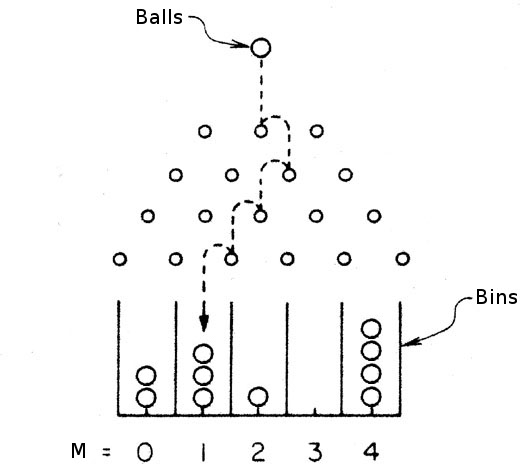
\includegraphics[width=\linewidth]{figures/BnB.jpeg}
	\caption{Balls-and-Bins \autocite{bnb}.}
	\label{fig:balls-and-bins}
\end{figure}
\par
Using the balls-and-bins approach we model processes as bins and events as balls and calculate how many balls need to be \textit{thrown} such that every bin contains at least one ball with arbitrarily high probability. With this approach the number of messages transmitted per process per round is logarithmic in the number of processes, therefore the number of messages sent in the system is low and uniform over all processes. Thanks to these approaches, \epto becomes highly scalable and resilient, while still providing total order.
\par
Until now, the creators of \epto have only tested this algorithm in a simulated environment. In this work, we implement \epto in pure Kotlin and introduce a benchmarking solution to show that \epto is suitable for real-world large-scale distributed systems. We compare \epto to the deterministic total order algorithm provided by \jgroups \autocite{jgroups} in both stable and unstable environments. \epto uses a PSS CYCLON \autocite{Voulgaris2005} to obtain a random view, coupled with a tracker that keeps track of dead and alive peers to obtain a first initial view. These benchmarks can easily be launched and scaled on a cluster using Docker and Docker Swarm. Furthermore, we can inject synthetic or real churn\footnote{Using the Failure Trace Archive databases} in the system.
\par
The next sections are dedicated to present our benchmarking solution and to present the results obtained. Section \ref{sec:ordering} presents the different kind of ordering. Section \ref{sec:definitions} defines the terms used in the paer. Section \ref{sec:epto} presents \epto and the architecture of our implementation. Section \ref{sec:evaluation} shows and explains the results obtained. We then argue about future work in section \ref{sec:future-work}. We finally draw conclusions in section \ref{sec:conclusion}.